\subsection{Introduction}
\indent The unique requirements for the sensor developed for deployment on the Claiborn Pell Newport Bridge set the sensor apart from off-the-shelf sensors readily available for purchase.
The sensor package needed to record high precision, high resolution accelerometer and strain gauge data continuously for an extended period of time. 
The longevity of the package was dependent upon the battery capacity and data storage capacity. 
This could have been solved by utilizing a large bank of batteries and multiple hard disk drives; however it was determined that this was a not a feasible option. 
Instead the sensor package would scavenge energy to recharge batteries and transmit data to a base station wirelessly. 
The addition of these two requirements greatly increased the complexity of the sensor package design. \\

\indent 

\subsection{Circuitry}

\subsubsection{Voltage Regulation}
The voltage input for most systems on the sensor board are a range of voltages between 3.3V-5V.
This posed a basic issue due to the output voltage of the 12V battery. 
The solution was to use two LM317 linear voltage regulators.
It was initially proposed to use the two regulators in series, such that the voltage dropped from 12V to 5V and then to 3.3V.
However, due to the current rating on the devices, it was decided to use the regulators in parallel and drop the voltage from 12V to 5V and 12V to 3.3V.
The complete circuit may be found in Figure \ref{fig:Schematic_VoltageReg}.
The LM317 technical specifications are displayed in Table \ref{tab:LM317} 

\begin{table}[h]
\centering
\begin{tabular}{|l|c|}
\hline
\textbf{Parameter} & \textbf{Value}\\
\hline
Input Voltage Differential ($V_{in}-V_{out}$)& 3V $\le V_{in}-V_{out} \le$ 40V\\
Output Voltage ($V_{out}$) & 1.2V $\le V_{out} \le$ 37V\\
Output Current ($I_{out}$) & 1.5A\\
Max Power Dissipation ($P_{D}$) & 20W\\
Package Type				   & TO-220\\
\hline
\end{tabular}
\caption{\textit{LM317 Adjustable Linear Regulator Specifications}}
\label{tab:LM317}
\end{table}

The output voltage can be set using Equation \ref{eqn:LM317} where $R_1= 240\Omega$ and $I_{adj}\le 100\mu A$.
It should be noted the $V$ is not the input voltage, but a unit placeholder.
Since $I_{adj}$ is very low, the error associated with it is almost negligible. 
\begin{equation}
V_{out} = 1.25V(1+\frac{R_2}{R_1}) + I_{adj}R_2
\label{eqn:LM317}
\end{equation}
The regulation circuit was tested using a 7.7Ah 12V battery in order to confirm the output voltages. %Possibly test and record range of input and output voltages
The voltages recorded were steady at approximately 3.5V and 5.3V.
The error is believed to be due to the inherent tolerance in the passive components used in the circuit.
Also in field use, the package will be subject to a wide range of temperatures that will cause the error in voltage to vary.

\subsubsection{ADC Impedance Matching}
\label{sec:ADC_Impedance_Matching}
As mentioned in Section \ref{sec:ADC_Impedance_Issues}, impedance matching issues were encountered when sampling accelerometer data with the micro-controller.
To avoid such issues in the final design, an impedance matching op-amp was used.
The MCP606 op-amp was used due to its rail-to-rail output, low input offset voltage, unity gain stability and low power characteristics. 
In order to act as a buffer for the input of the ADC, the op-amp was configured as in Figure \ref{fig:op-amp_standard}; where $R_1$ and $R_2$ are governed by the Equation \ref{eqn:op-amp_gain}. 
Since the op-amp will be used with unity gain (gain = 1) then both resistors are $0\Omega$ and just wired connections \cite{ArtofElectronics}.

\begin{figure}
\centering
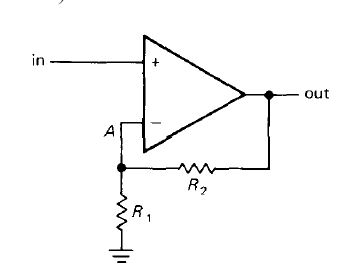
\includegraphics[scale=1]{Op-Amp_Standard}
\caption{Standard configuration of op-amp as a buffer}
\label{fig:op-amp_standard}
\end{figure}

\begin{equation}
gain = 1 + \frac{R_{2}}{R_{1}}
\label{eqn:op-amp_gain}
\end{equation}

\subsubsection{Decoupling Capacitors}
In order to reduce noise on the power supply line to each component, decoupling capacitors were added to each device between the voltage input and ground.
Decoupling capacitors act as low-pass filters, thus removing high frequency voltage differentials.
To ensure no inductance due to the transmission length between the decoupling capacitors and device inputs, the transmission length was minimized \cite{ArtofElectronics}.


\subsection{Printed Circuit Board}
\label{sec:PCB}
In order to combine the system in an efficient manor, it was decided that a printed circuit board (PCB) must be designed to carry the components.
This would make future sensor packages easy to manufacture for additional sensor nodes on the bridge and ensures consistency between packages.
It should be noted that all schematics and circuit board files were created using National Instruments Multisim 13.0 and Ultiboard 13.0 respectfully.
All schematics and board files may be found at \url{https://github.com/mpiannucci/SeniorDesign/tree/master/hardware}.
 
\subsubsection{Requirements for PCB}
Initially the requirements for the PCB were to create a carrier board that would allow for the addition and removal of package components via header sockets.
This would allow for the purchase of many off-the-shelf components that would be able to be installed with minimal effort.
For various reasons, the scope of the PCB was change from being a carrier board to completely integrating all of the components.
This posed difficulties as many of the components utilized in the package were bought as standalone solutions with dedicated PCBs for each component.
As a solution for this, all component that shipped with PCBs had all of their circuitry mimicked on the main PCB.
This holds true for all components except for three; BeagleBone Black, Trimble Copernicus II GPS receiver and the XBee Pro S3B wireless receiver.
It was decided that it was more appropriate to create sockets for each of these components to plug into for specific reasons.
Although the board files for the BeagleBone Black are readily available to download, it was deemed unnecessary to recreate the board.
For the Trimble Copernicus II GPS receiver, it was decided that because of the sensitivity in the design of the antenna circuit that it would be best to use the off-the-shelf board.
The board purchased has the antenna circuit integrated with impedance matched SMA connector for the antenna.
Due to unforeseen issues with interfacing the XBee Pro S3B wireless receivers, the receiver was not incorporated in the initial version of the system design.
Section \ref{sec:XBeeFuture} discusses the future work to be done with the XBee Pro S3B receivers.

\subsubsection{Progress on Printed Circuit Board}
All component footprints for components in the sensor package were created in Multisim 13.0 and Ultiboard 13.0.
The library of components may be found at \url{https://github.com/mpiannucci/SeniorDesign.git} under \verb|./hardware/UsrComp_S_SHMComps.usr|.
A basic board was laid out, however trace routing was not completed due to unresolved net issues.
Although the board design was not finished, a comprehensive schematic was created and will prove useful for future development of the board.
The schematics may be found in Appendix \ref{app:Schematic}.